\documentclass[11pt]{article}
\usepackage[margin=1in]{geometry}
\usepackage{amsmath,amssymb,amsthm}
\usepackage{graphicx}
\usepackage[hidelinks]{hyperref}

\newtheorem{theorem}{Theorem}

\newcommand{\D}{\mathbb D}
\newcommand{\C}{\mathbb C}
\newcommand{\B}{\mathcal B}
\newcommand{\A}{\mathcal A}
\newcommand{\calL}{\mathcal L}
\newcommand{\Lat}{\operatorname{Lat}}
\newcommand{\ran}{\operatorname{ran}}
\newcommand{\kerop}{\operatorname{ker}}

\title{A Complemented-Kernel Partial Result for arXiv:2406.02330}
\author{Run \texttt{fa\_banach\_001}, agent \texttt{agent\_lane\_01}}
\date{2026-07-03}

\begin{document}
\maketitle

\section*{Source And Target}

The source paper is L. Abadias, F. J. Gonzalez-Dona, and J. Oliva-Maza,
\emph{Universality arising from invertible weighted composition operators},
arXiv:2406.02330.

In Section 5 the authors pass from Hilbert spaces to the Banach spaces
\[
  \B=H^p \quad\text{or}\quad \B=\A_\sigma^p,
  \qquad 1\le p<\infty,\quad \sigma>-1.
\]
Let \(uC_\psi\) be an invertible weighted composition operator with hyperbolic
symbol \(\psi\), with attractive and repulsive fixed points \(a,b\), and let
\[
 A^+=\limsup_{z\to a}|u(z)|,\quad A^-=\liminf_{z\to a}|u(z)|,\quad
 B^+=\limsup_{z\to b}|u(z)|,\quad B^-=\liminf_{z\to b}|u(z)|.
\]
The parameter \(\gamma\) is \(1/p\) for \(H^p\) and \((\sigma+2)/p\) for
\(\A_\sigma^p\).  Under
\[
  \frac{B^+}{(\psi'(b))^\gamma}<\frac{A^-}{(\psi'(a))^\gamma}
\]
and
\[
  \frac{B^+}{(\psi'(b))^\gamma}<|\lambda|<
  \frac{A^-}{(\psi'(a))^\gamma},
\]
the source asks whether \(\ker(uC_\psi-\lambda I)\) is complemented and
contains a subspace isomorphic to \(\B\).

\begin{center}
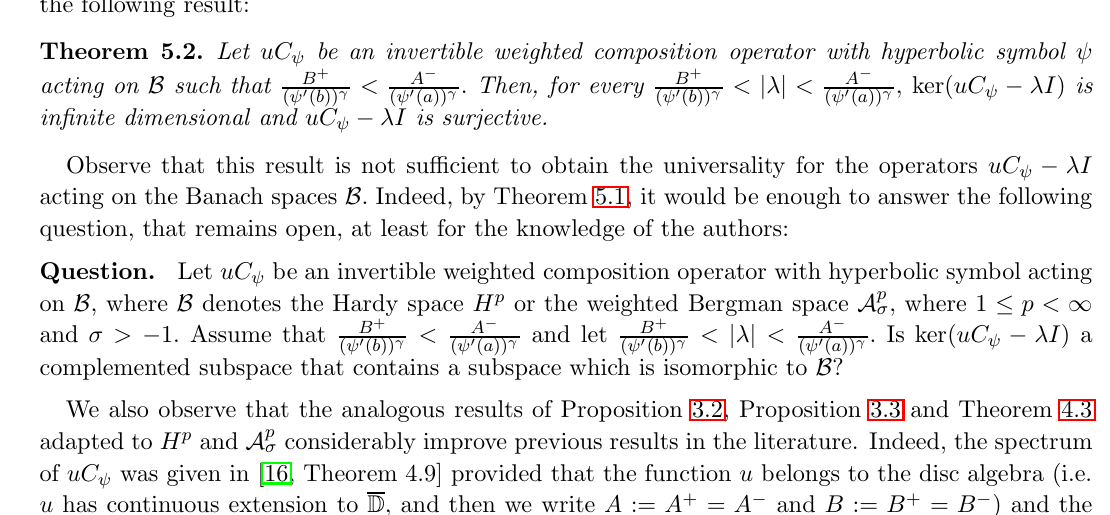
\includegraphics[width=.92\linewidth]{figures/banach_question_crop.png}
\end{center}

\section*{Result}

We prove the complementability half of the question.

\begin{theorem}
Under the hypotheses above, the operator
\[
  S_\lambda=\lambda I-uC_\psi:\B\to\B
\]
has a bounded right inverse. Consequently
\[
  \ker(uC_\psi-\lambda I)=\ker S_\lambda
\]
is a complemented subspace of \(\B\).
\end{theorem}

\section*{Proof Intuition}

The source already proves that \(S_\lambda\) is onto \(\B\), but it does so by
solving the equation separately on two range spaces
\(\B_{\mu,0}\) and \(\B_{0,\nu}\), then using the algebraic decomposition
\(\B=\B_{\mu,0}+\B_{0,\nu}\).  The small extra observation is that this
decomposition can be chosen by a bounded linear formula.  Therefore the two
bounded inverses on the range spaces glue into a bounded right inverse on
\(\B\).  A bounded right inverse immediately gives a projection onto the
kernel.

\section*{Proof}

For \(\mu,\nu\ge0\), set
\[
  \omega_{\mu,\nu}(z)=(a-z)^\mu(b-z)^\nu,\qquad
  \B_{\mu,\nu}=\omega_{\mu,\nu}\B
\]
with norm \(\|f\|_{\B_{\mu,\nu}}=\|f/\omega_{\mu,\nu}\|_{\B}\).  Multiplication
by \(\omega_{\mu,\nu}\) identifies \(\B\) isometrically with
\(\B_{\mu,\nu}\), and the inclusion \(\B_{\mu,\nu}\hookrightarrow \B\) is
bounded.

Choose \(\mu,\nu>0\) as in the proof of Theorem 4.1 of the source, adapted in
Section 5 to the Banach spaces: namely,
\[
  |\lambda|>A^+(\psi'(a))^{\mu-\gamma},
  \qquad
  |\lambda|<B^-(\psi'(b))^{\nu-\gamma}.
\]
The source argument shows that \(S_\lambda\) is boundedly invertible on
\(\B_{\mu,0}\) and on \(\B_{0,\nu}\).  Denote these bounded inverses by
\[
  R_\mu:\B_{\mu,0}\to\B_{\mu,0},
  \qquad
  R_\nu:\B_{0,\nu}\to\B_{0,\nu}.
\]

It remains only to keep track of the splitting.  Pick integers \(m,n\) with
\(m\ge\mu\) and \(n\ge\nu\).  For \(f\in\B\), the binomial identity gives
\[
f(z)=\frac{1}{(a-b)^{m+n}}
 \sum_{j=0}^{m+n} \binom{m+n}{j}(-1)^{m+n-j}
 (a-z)^j(b-z)^{m+n-j}f(z).
\]
Define
\[
  Pf=\frac{1}{(a-b)^{m+n}}
 \sum_{j=m}^{m+n} \binom{m+n}{j}(-1)^{m+n-j}
 (a-z)^j(b-z)^{m+n-j}f
\]
and
\[
  Qf=\frac{1}{(a-b)^{m+n}}
 \sum_{j=0}^{m-1} \binom{m+n}{j}(-1)^{m+n-j}
 (a-z)^j(b-z)^{m+n-j}f .
\]
Then \(P,Q:\B\to\B\) are bounded linear maps, \(P+Q=I_\B\),
\(\ran P\subseteq\B_{\mu,0}\), and \(\ran Q\subseteq\B_{0,\nu}\).

Now set
\[
  R=R_\mu P+R_\nu Q:\B\to\B .
\]
This operator is bounded, and
\[
  S_\lambda Rf
  =S_\lambda R_\mu Pf+S_\lambda R_\nu Qf
  =Pf+Qf=f
\]
for every \(f\in\B\).  Hence \(R\) is a bounded right inverse for
\(S_\lambda\).

Finally,
\[
  \Pi=I_\B-RS_\lambda
\]
is a bounded projection onto \(\ker S_\lambda\): indeed
\[
  S_\lambda\Pi=S_\lambda-S_\lambda R S_\lambda=0,
\]
so \(\ran\Pi\subseteq\ker S_\lambda\), while \(\Pi x=x\) for every
\(x\in\ker S_\lambda\).  Thus \(\ker(uC_\psi-\lambda I)\) is complemented.
\qed

\section*{Limitations And Novelty Check}

This does not prove that the kernel contains a subspace isomorphic to
\(\B\), so it does not by itself prove Banach-space universality via the
Banach Caradus criterion.  It reduces the source question to the
copy-of-\(\B\) part.

The run's lightweight indexes had no exact prior packet for arXiv:2406.02330.
An exact web search for the complemented-kernel phrasing found the source
arXiv record and no separate answer.

\section*{References}

\begin{thebibliography}{9}
\bibitem{source}
L. Abadias, F. J. Gonzalez-Dona, and J. Oliva-Maza,
\emph{Universality arising from invertible weighted composition operators},
arXiv:2406.02330.

\bibitem{Caradus}
S. R. Caradus,
\emph{Universal operators and invariant subspaces},
Proc. Amer. Math. Soc. 23 (1969), 526--527.
\end{thebibliography}

\end{document}
